\section{Bayesian Analysis}
\label{sec:bayesian}
\label{app:ext_bayes}
\emph{In short: the same likelihood with uniform priors, sampled with MCMC: $\Araw=-0.0443$ ($68\%$ interval $[-0.0528,-0.0358]$) with converged chains; the Bayes factor of $A=0$, $BF_{10}\approx9\times10^3$, depends on the prior width.}
The Bayesian analysis takes the likelihood of Sec.~\ref{sec:model} as it is and adds only a prior and a sampler; it changes the question asked of the data, not the model.

\subsection{Priors and Posterior}
\label{sec:bayes_prior}
\emph{In short: uniform bounded priors on twelve parameters; with $\sim2\times10^4$ candidates the posterior is dominated by the likelihood.}
Bayes' theorem combines the likelihood of Eq.~\eqref{eq:likelihood} (Sec.~\ref{sec:model}) with a prior $\pi(\theta)$ into the posterior
\begin{equation}
p(\theta\mid D)=\frac{\mathcal{L}(D\mid\theta)\,\pi(\theta)}{p(D)},
\label{eq:bayes}
\end{equation}
The priors are uniform, with independent ranges except for the ordering of the background slopes: $N_s,N_b\in(0,5N)$ with $N=19{,}731$, $A,A_b\in(-1,1)$, $\mu\in(5260,5310)\,\MeV$, $\sigma\in(3,40)\,\MeV$, $\lambda_1^{\pm}\in(10^{-5},0.1)\,\MeV^{-1}$, $\lambda_2^{\pm}\in(10^{-5},\lambda_1^{\pm})$, $f_{\pm}\in(0,1)$. The prior density is therefore a constant on the allowed region $\Theta$,
\begin{equation}
\pi(\theta)\propto\mathbf{1}\left[\theta\in\Theta\right],
\label{eq:prior}
\end{equation}
and inside it the posterior is proportional to the likelihood. With $\sim$$2\times10^4$ events the posterior is dominated by the likelihood, as the prior-sensitivity check confirms for $A$. The evidence $p(D)$ is a constant: the MCMC samples $\mathcal{L}\,\pi$ without it, and the Savage-Dickey ratio of Sec.~\ref{sec:bayes_factor} avoids it as well; the marginal posterior of $A$ is the histogram of the $A$ component of the chain.

\subsection{MCMC Sampling and Convergence Diagnostics}
\label{sec:bayes_mcmc}
\emph{In short: 32 walkers for $25{,}000$ steps; the chain is at least $113$ autocorrelation times long for every parameter and independent runs from dispersed starting points agree.}
The posterior was sampled with the affine-invariant ensemble sampler of Goodman and Weare~\cite{goodman_weare} as implemented in \texttt{emcee}~\cite{emcee} (Sec.~\ref{app:theory}): 32 walkers started around the maximum of the posterior, $25{,}000$ steps with the first $1/6$ discarded as burn-in ($6.7\times10^5$ samples, acceptance $0.38$). The integrated autocorrelation time is $\tau\in[147,183]$ steps, so the chain is $N/\tau\geq113$ autocorrelation times long for every parameter, above the threshold of $50$~\cite{emcee} ($\gtrsim3600$ effectively independent samples). Two runs started uniformly over the whole prior box converge to the same single mode ($\Araw=-0.0446$ and $-0.0442$; trace plot in Fig.~\ref{fig:bayes_trace}).

\subsection{Posterior Results and Credible Intervals}
\label{sec:bayes_posterior}
\emph{In short: $\Araw=-0.0443$, 68\% credible interval $[-0.0528,-0.0358]$ and 95\% $[-0.0608,-0.0276]$; the posterior is Gaussian.}
\begin{figure*}[!t]
\centering
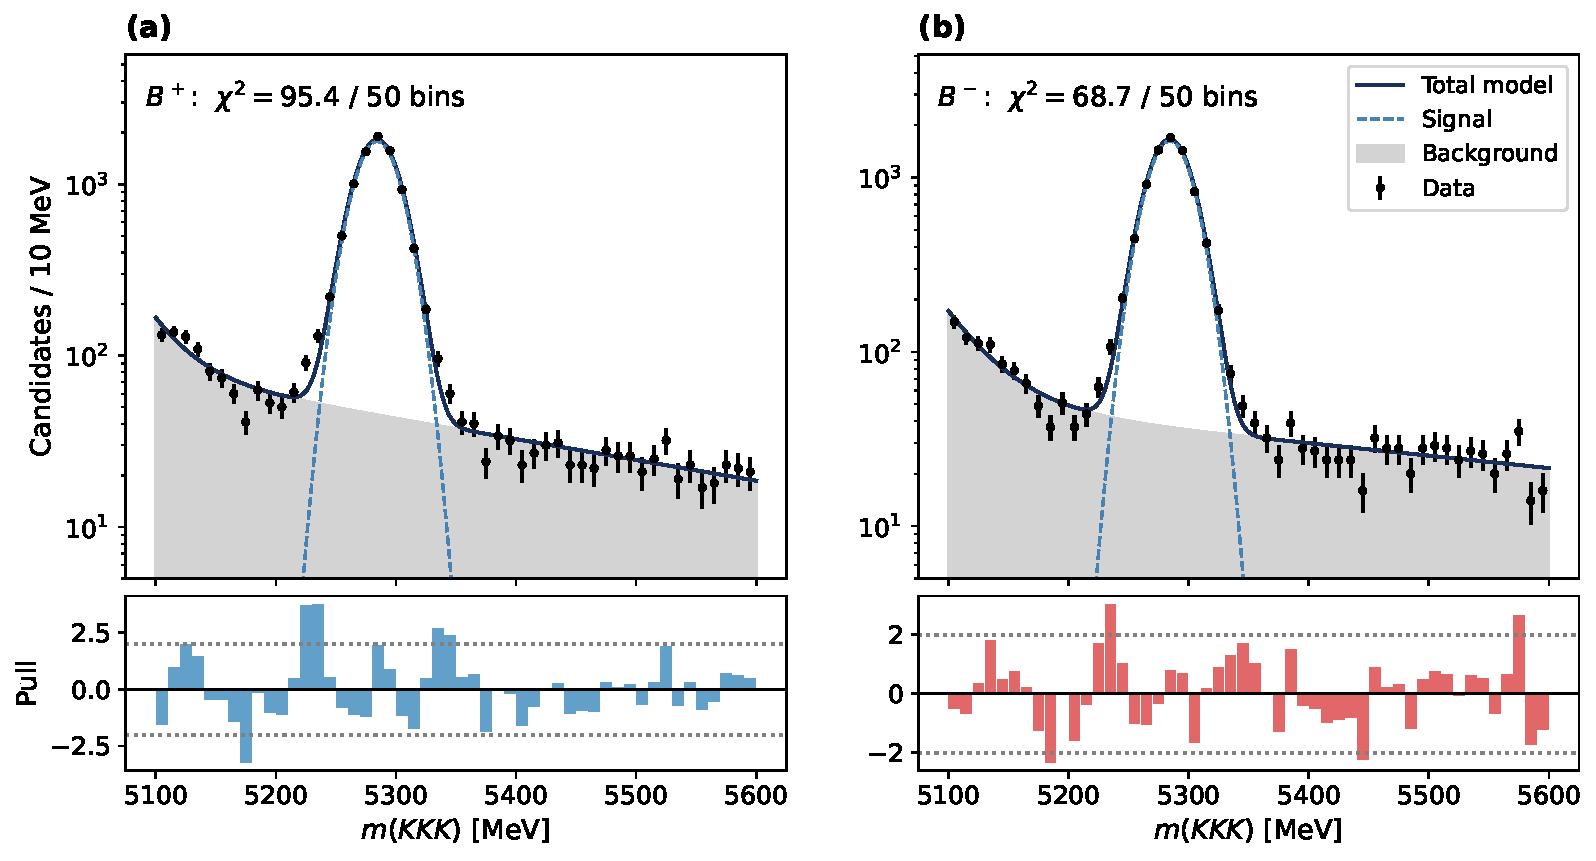
\includegraphics[width=0.8\textwidth]{figures/bayes_nominal_mass_fit.pdf}
\caption{Mass distributions of (a) $B^+$ and (b) $B^-$ candidates with the nominal model (posterior medians, logarithmic scale): total, signal and background components. Bottom: pulls, $(\text{obs}-\text{exp})/\sqrt{\text{exp}}$.}
\label{fig:bayes_fit}
\end{figure*}

\begin{figure*}[t]
\centering
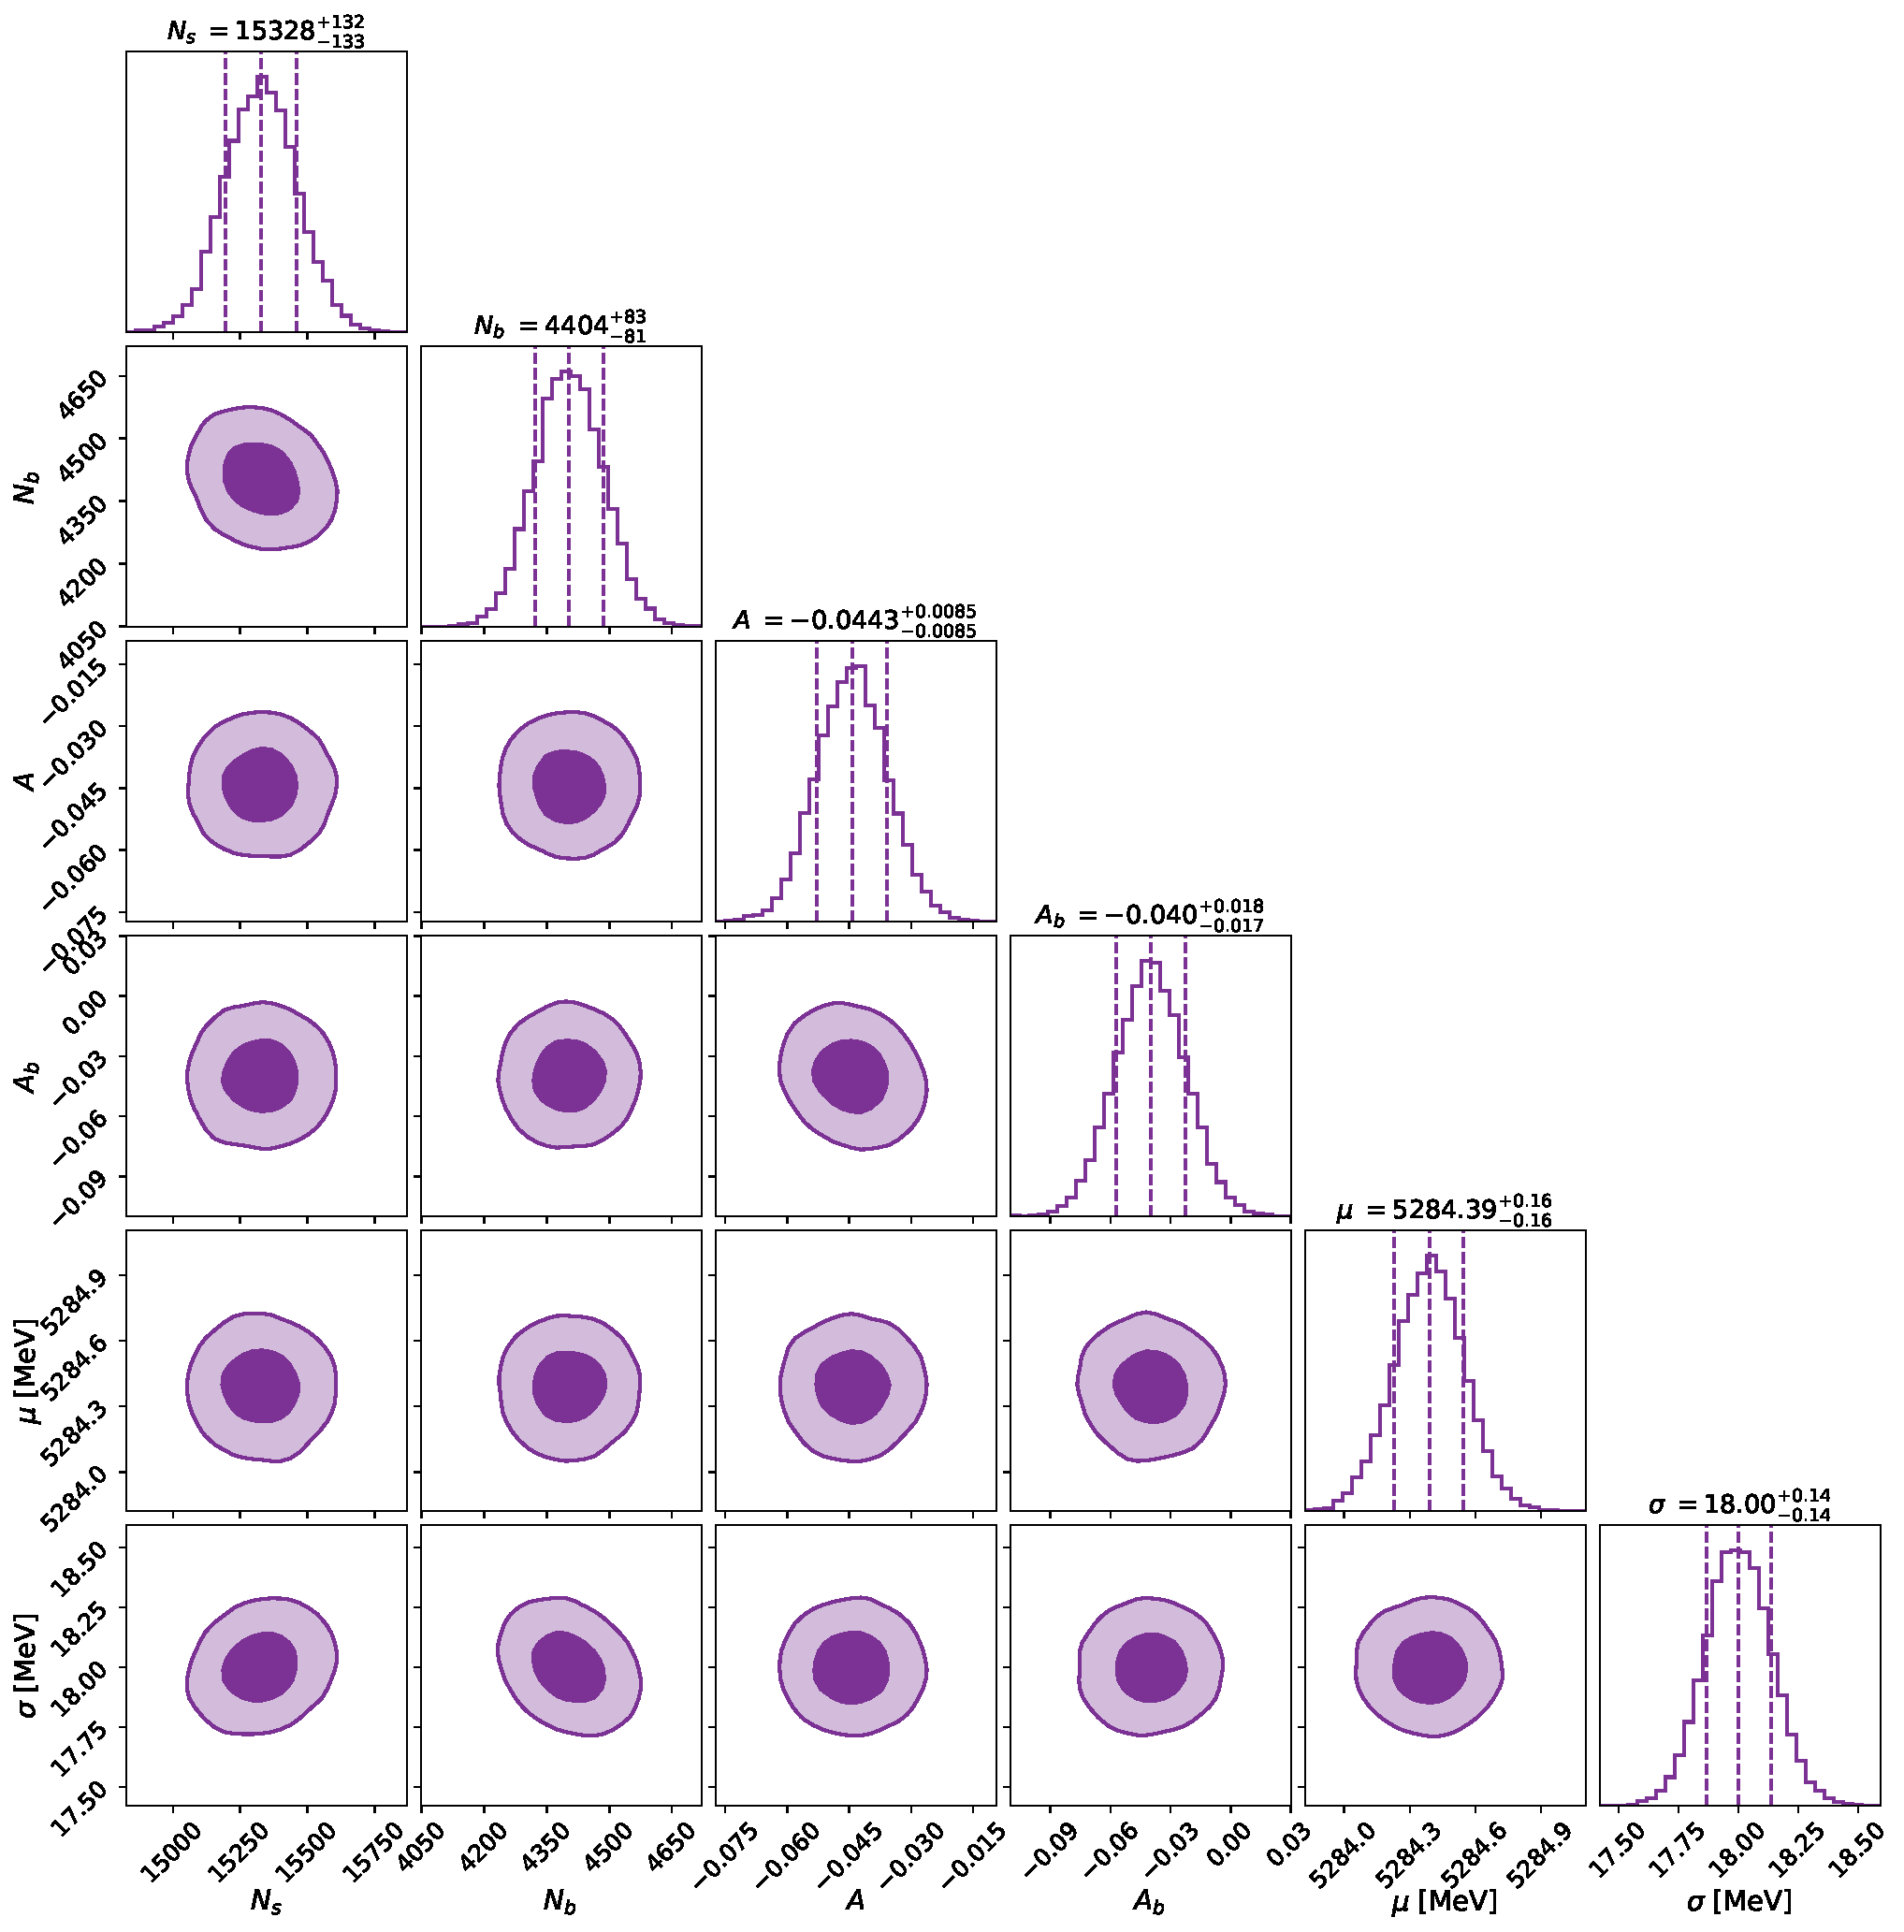
\includegraphics[width=0.55\textwidth]{figures/bayes_nominal_corner.pdf}
\caption{Posterior of the six physics parameters of the nominal fit (the six background-shape parameters are marginalized). Diagonal: marginal posteriors with the 16th, 50th and 84th percentiles (dashed lines and titles). Off-diagonal: 2D marginals, contours enclosing the regions of the $1\sigma$ and $2\sigma$ levels of a 2D Gaussian ($39\%$ and $86\%$).}
\label{fig:bayes_corner}
\end{figure*}

Figure~\ref{fig:bayes_fit} compares the nominal model with the data of the two charges: it follows the spectrum over two orders of magnitude, and the pulls show signal tails heavier than a Gaussian, whose effect on $\Araw$ is negligible (Sec.~\ref{sec:bayes_gof}). The marginal posterior on the raw asymmetry gives (median and equal-tailed credible intervals, CI)
\begin{gather*}
\Araw = -0.0443, \\
68\%~\text{CI}~[-0.0528,-0.0358], \\ 95\%~\text{CI}~[-0.0608,-0.0276].
\end{gather*}
The posterior is very close to Gaussian (standard deviation $0.0085$), so equal-tailed and highest-posterior-density intervals coincide; with uniform priors its mode, $-0.0441$, is the maximum-likelihood estimate and the result can be compared directly with the Frequentist fit (Secs.~\ref{sec:frequentist} and~\ref{sec:appendix_freq}). The other physics parameters (Fig.~\ref{fig:bayes_corner}) are $N_s=15{,}328\pm133$, $N_b=4404\pm82$, $A_b=-0.040\pm0.018$, $\mu=5284.39\pm0.16\,\MeV$ and $\sigma=18.00\pm0.14\,\MeV$. $A$ is almost uncorrelated with them, which is why profiling (Frequentist) and marginalizing (Bayesian) the nuisance parameters give the same result; the largest correlation, $-0.17$, is with $A_b$: conditioning on $A_b=0$ moves $A$ to $-0.0475$, as the fit with a charge-symmetric background does ($-0.0471$, Sec.~\ref{sec:syst}).




\subsection{Bayes Factors}
\label{sec:bayes_factor}
\emph{In short: decisive evidence against $A=0$ (Bayes factor $BF_{10}\approx9\times10^3$); the evidence for a background asymmetry is not significant, and depends on the prior width.}

The Bayes factor compares two hypotheses through their evidences, $BF_{10}=P(D\mid H_1)/P(D\mid H_0)$, and requires proper priors. For the nested hypothesis $H_0$: $A=0$ against $H_1$: $A$ free, with shared priors on the other parameters, it reduces to the Savage-Dickey ratio~\cite{dickey1971} (Sec.~\ref{sec:appendix_freq}),
\[
BF_{01} = \frac{p(A=0\mid D)}{\pi(A=0)}, \qquad \pi(A=0)=\tfrac12 .
\]
$A=0$ lies $5.2$ posterior standard deviations from the median, where the chain has essentially no samples, so $p(A=0\mid D)$ was taken from the Gaussian approximation of the marginal posterior: $BF_{01}\approx1.1\times10^{-4}$ ($BF_{10}\approx9\times10^{3}$), decisive evidence against $A=0$ on Jeffreys' scale~\cite{jeffreys}. The value scales with the prior width (Ockham factor): with $A\in(-0.3,0.3)$, $BF_{01}$ drops by a factor $3.3$ and the conclusion is unchanged (Fig.~\ref{fig:checks_bf}; the Savage-Dickey densities are in Fig.~\ref{fig:bayes_sd}, further checks in Sec.~\ref{sec:checks_profile}).

\begin{figure}[h]
\centering
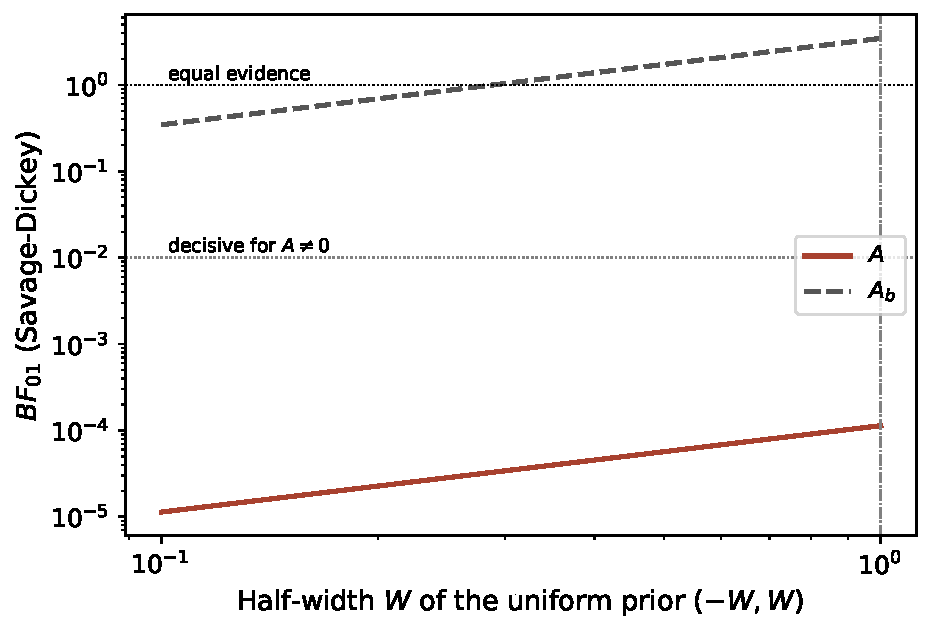
\includegraphics[width=\columnwidth]{figures/validation_bf_prior_width.pdf}
\caption{$BF_{01}$ of $A=0$ and of $A_b=0$ as a function of the half-width $W$ of the uniform prior $(-W,W)$ (Gaussian approximation of the posterior, Savage-Dickey). The vertical line marks the nominal prior.}
\label{fig:checks_bf}
\end{figure}


The same test on the background asymmetry shows the Ockham factor at work: $A_b=-0.040\pm0.018$ is $2.3$ standard deviations from zero, yet $BF_{01}(A_b=0)\approx3.5$, because the likelihood gain does not compensate for spreading the prior over $(-1,1)$; unlike for $A$, the preference changes sign with the prior width (Fig.~\ref{fig:checks_bf}, crossing at $W\approx0.3$). Of the Bayesian results only the Bayes factor depends on the prior; the interval of $A$ does not (Sec.~\ref{sec:bayes_posterior}). A negative $A_b$ is plausible given the misidentified $B^\pm\to K^\pm\pi^+\pi^-$ and $\pi^\pm K^+K^-$ decays; $A_b$ is kept free in the nominal model and fixing it to zero is one of the systematic variants (Sec.~\ref{sec:syst}).

 \emph{Model Adequacy: Goodness of Fit and Posterior Predictive Check}: the model does not reach $\chi^2/\mathrm{ndof}\approx1$ ($164.1/88$), mainly because the signal tails are heavier than a Gaussian, but $\Araw$ changes by only $-0.0002$ with a Crystal Ball signal.

\subsection{Metropolis-Hastings and the Ensemble Sampler}
\label{app:theory}
\emph{In short: Metropolis-Hastings accepts a proposal with a ratio that satisfies detailed balance; the affine-invariant ensemble move samples correlated posteriors without tuning, and $N/\tau$ is the effective length of a chain.}
The Metropolis-Hastings algorithm builds a Markov chain whose stationary distribution is the target $\pi(\theta)$: from the state $x$ a point $y$ is proposed from $q(y\mid x)$ and accepted with probability $\min\!\big[1,\pi(y)\,q(x\mid y)/(\pi(x)\,q(y\mid x))\big]$, which satisfies detailed balance. Its efficiency depends on how the proposal is matched to the (here correlated) posterior. The ensemble sampler used for the nominal fit~\cite{goodman_weare,emcee} evolves $K$ walkers; to update the walker $X_k$ it picks another walker $X_j$ and proposes $Y=X_j+Z\,(X_k-X_j)$, with $Z\in[1/a,a]$ drawn from $g(z)\propto z^{-1/2}$ ($a=2$), and accepts it with probability $\min\!\big[1,Z^{d-1}\pi(Y)/\pi(X_k)\big]$ ($d$ the number of parameters). The move is invariant under affine transformations of the parameters, so a strongly correlated, elongated posterior is as easy to sample as a spherical one, and it needs no hand-tuned proposal covariance.

Successive states of a chain are correlated. The integrated autocorrelation time of a parameter is $\tau=1+2\sum_{t\geq1}\rho(t)$, with $\rho(t)$ the autocorrelation of the chain at lag $t$, and a chain of $N$ steps contains $N_{\mathrm{eff}}=N/\tau$ effectively independent samples, so that the Monte Carlo error of a posterior mean is $\sigma/\sqrt{N_{\mathrm{eff}}}$. The estimate of $\tau$ is itself reliable only for $N\gtrsim50\,\tau$~\cite{emcee}.

\subsection{Sampling and Convergence Diagnostics}
\emph{In short: $32$ walkers for $25{,}000$ steps give $N/\tau\geq113$ autocorrelation times for every parameter, and runs started over the whole prior box converge to the same single mode.}
The posterior was sampled with the affine-invariant ensemble sampler of Goodman and Weare~\cite{goodman_weare} as implemented in \texttt{emcee}~\cite{emcee} (the stretch move, the autocorrelation time and the effective sample size are described in Sec.~\ref{app:theory}). The maximum of the posterior was first located numerically (Nelder-Mead), and 32 walkers were initialized in a narrow ball around it and run for $25{,}000$ steps, with the first $4166$ ($1/6$) discarded as burn-in, leaving $6.7\times10^5$ samples; the mean acceptance fraction is $0.38$. Convergence was checked through the integrated autocorrelation time of each parameter, $\tau=1+2\sum_{t\geq1}\rho(t)$, with $\rho(t)$ the autocorrelation of the chain at lag $t$. We find $\tau\in[147,183]$ steps, the longest for the background-shape parameters: the post-burn-in chain is $N/\tau\geq113$ autocorrelation times long for every parameter, above the threshold of $50$ recommended for a reliable estimate of $\tau$~\cite{emcee}, and corresponds to $\gtrsim3600$ effectively independent samples per parameter. To check that the chain is not trapped near its starting point, the fit was repeated twice with the walkers initialized uniformly over the whole prior box and the first half of the chain discarded: both runs converge to the same single mode, with $\Araw=-0.0446$ and $-0.0442$, the same intervals and the same values of all other parameters as the nominal fit. The trace plot of such a run (Fig.~\ref{fig:bayes_trace}) shows all walkers reaching the bulk of the posterior within $\sim$2000 steps, the background fraction $f_+$ last, well inside the discarded half of the chain.

\begin{figure*}[t]
\centering
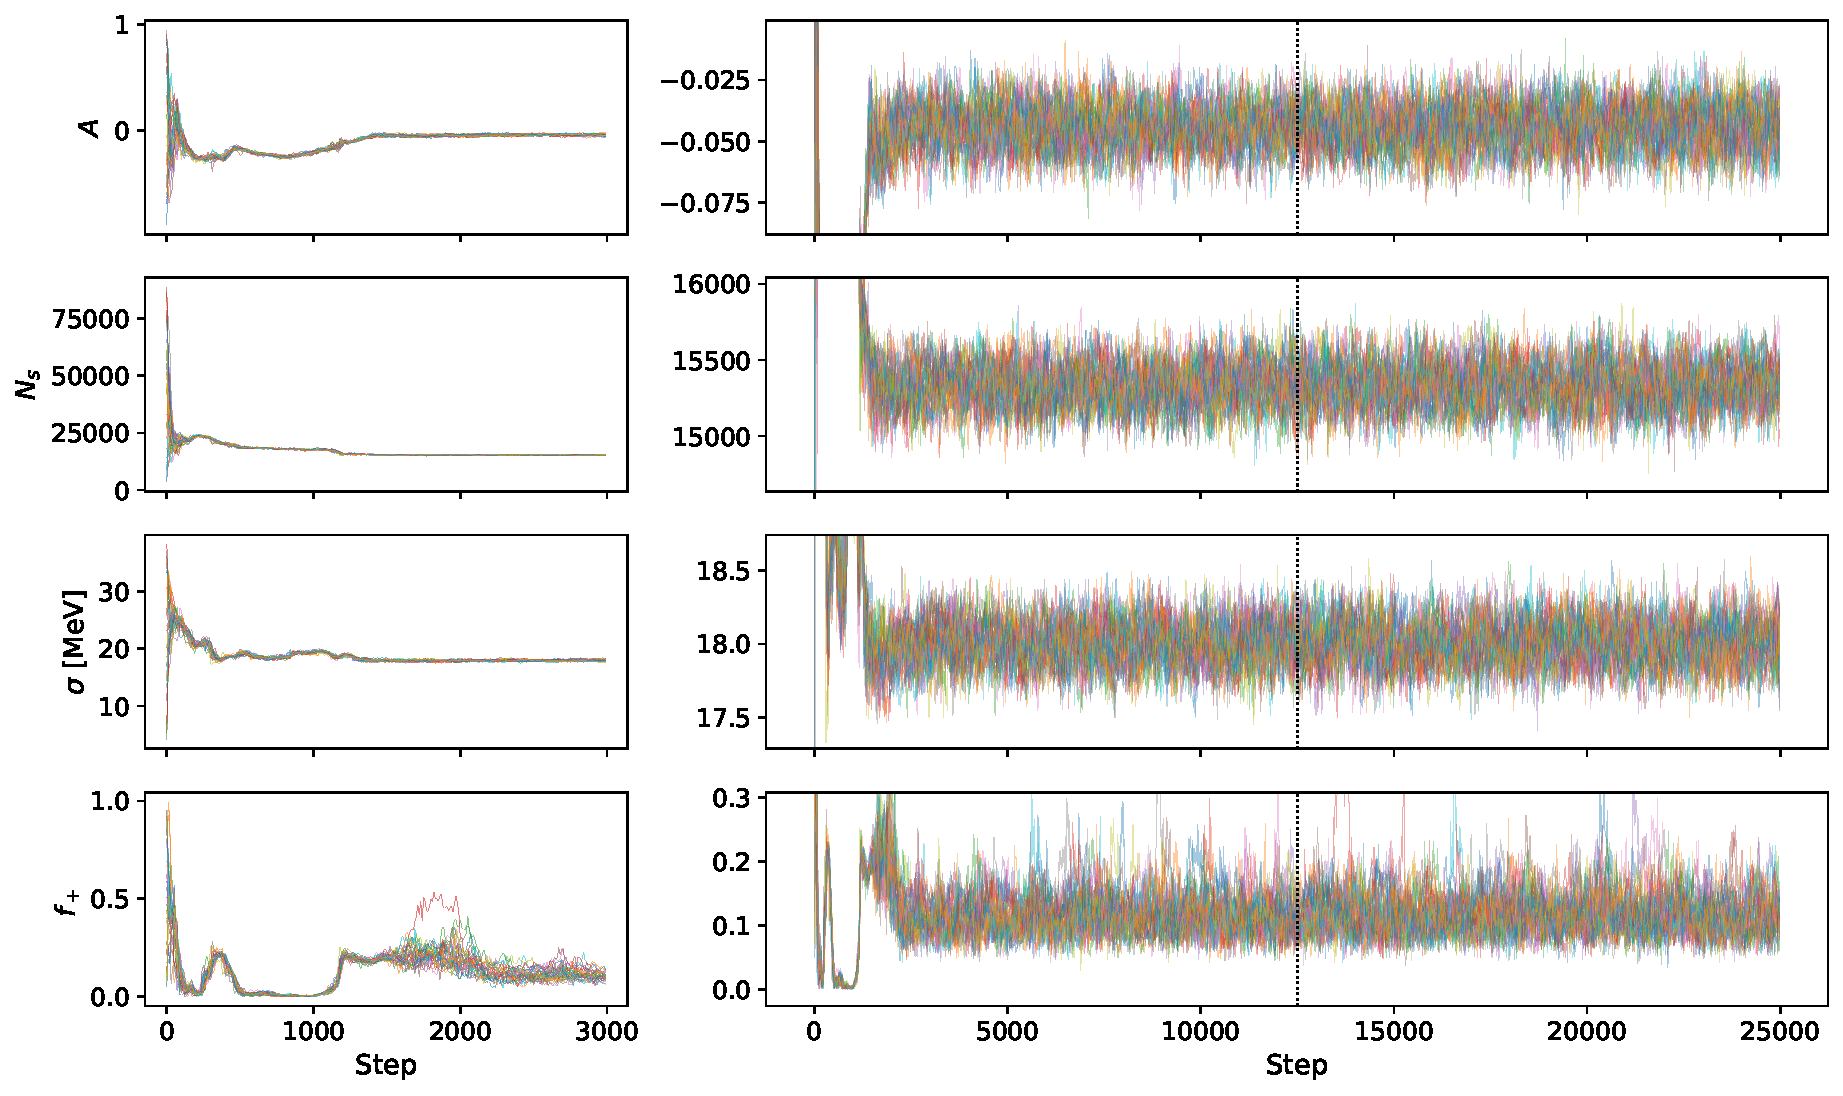
\includegraphics[width=0.95\textwidth]{figures/bayes_nominal_trace.pdf}
\caption{Trace plot of the nominal fit with the 32 walkers initialized uniformly over the prior box (one line per walker, every 10th step), for $A$, $N_s$, $\sigma$ and the steep-background fraction $f_+$. Left: first 3000 steps, full range; right: whole chain, zoomed on the posterior. The first half of the chain (dotted line) is discarded as burn-in.}
\label{fig:bayes_trace}
\end{figure*}

\subsection{Equal-Tailed and Highest-Posterior-Density Intervals}
\label{sec:checks_hpd}
\emph{In short: for $A$ and $A_b$ the two kinds of $68\%$ interval coincide; they differ for the skewed parameters, whose highest-posterior-density interval is shifted towards the mode.}
Table~\ref{tab:checks_hpd} compares the equal-tailed interval (percentiles $15.9\%$--$84.1\%$) with the interval of highest posterior density, the shortest containing $68.3\%$, for the parameters of interest and for three skewed nuisance parameters.

\begin{table}[h]
\centering
\resizebox{\ifdim\width>\linewidth\linewidth\else\width\fi}{!}{\begin{tabular}{lcccc}
\toprule
Parameter & median & equal-tailed & HPD & skewness \\
\midrule
$A$ & $-0.0442$ & $[-0.0529,-0.0358]$ & $[-0.0525,-0.0355]$ & $+0.01$ \\
$A_b$ & $-0.0400$ & $[-0.0575,-0.0224]$ & $[-0.0575,-0.0225]$ & $+0.01$ \\
$f_+$ & $0.114$ & $[0.089,0.145]$ & $[0.084,0.138]$ & $+0.90$ \\
$f_-$ & $0.209$ & $[0.174,0.248]$ & $[0.168,0.241]$ & $+0.33$ \\
$\lambda_1^+$ [MeV$^{-1}$] & $0.0350$ & $[0.0281,0.0431]$ & $[0.0274,0.0423]$ & $+0.52$ \\
\bottomrule
\end{tabular}}
\caption{Equal-tailed and highest-posterior-density $68\%$ intervals and skewness of the marginal posteriors.}
\label{tab:checks_hpd}
\end{table}

\subsection{Posterior Summaries and Model Comparison}
\emph{In short: equal-tailed and HPD intervals, the Jeffreys scale for Bayes factors, the Ockham effect of the prior width and the definition of the posterior predictive $p$-value.}
The credible intervals quoted are the equal-tailed ones (the $16\%$--$84\%$ quantiles for $68\%$); the highest-posterior-density (HPD) interval is the shortest interval with the same probability and coincides with it for a symmetric posterior. A Bayes factor $BF_{ij}=P(D\mid H_i)/P(D\mid H_j)$ is interpreted with the Jeffreys scale~\cite{jeffreys,kass_raftery}: values between $1$ and $3$ are barely worth mentioning, $3$--$10$ substantial, $10$--$30$ strong, $30$--$100$ very strong and above $100$ decisive. The evidence automatically penalizes unnecessary freedom (Ockham's razor): for a Gaussian posterior much narrower than a uniform prior of width $2W$ the Savage-Dickey ratio of $A=0$ is proportional to $W$, so widening the prior of $A$ favors the null hypothesis by construction, which is why the dependence on $W$ is reported.

The posterior predictive check compares the data $y$ with replicas $y^{\mathrm{rep}}$ simulated from the model at parameters drawn from the posterior, through a discrepancy statistic $T$: the posterior predictive $p$-value is $p_B=P\big(T(y^{\mathrm{rep}},\theta)\geq T(y,\theta)\mid y\big)$~\cite{gelman_ppc}. Values close to $0$ or $1$ signal a feature of the data that the model does not reproduce; a statistic that the fit adjusts directly (for example the total asymmetry, when $A$ is a free parameter) is reproduced by construction and tests nothing.

\subsection{Savage--Dickey Densities of the Parameters}
\label{app:sd_densities}
\emph{In short: the posterior and prior densities at the null value, which give the Bayes factors of the main text.}
\begin{figure*}[!t]
\centering
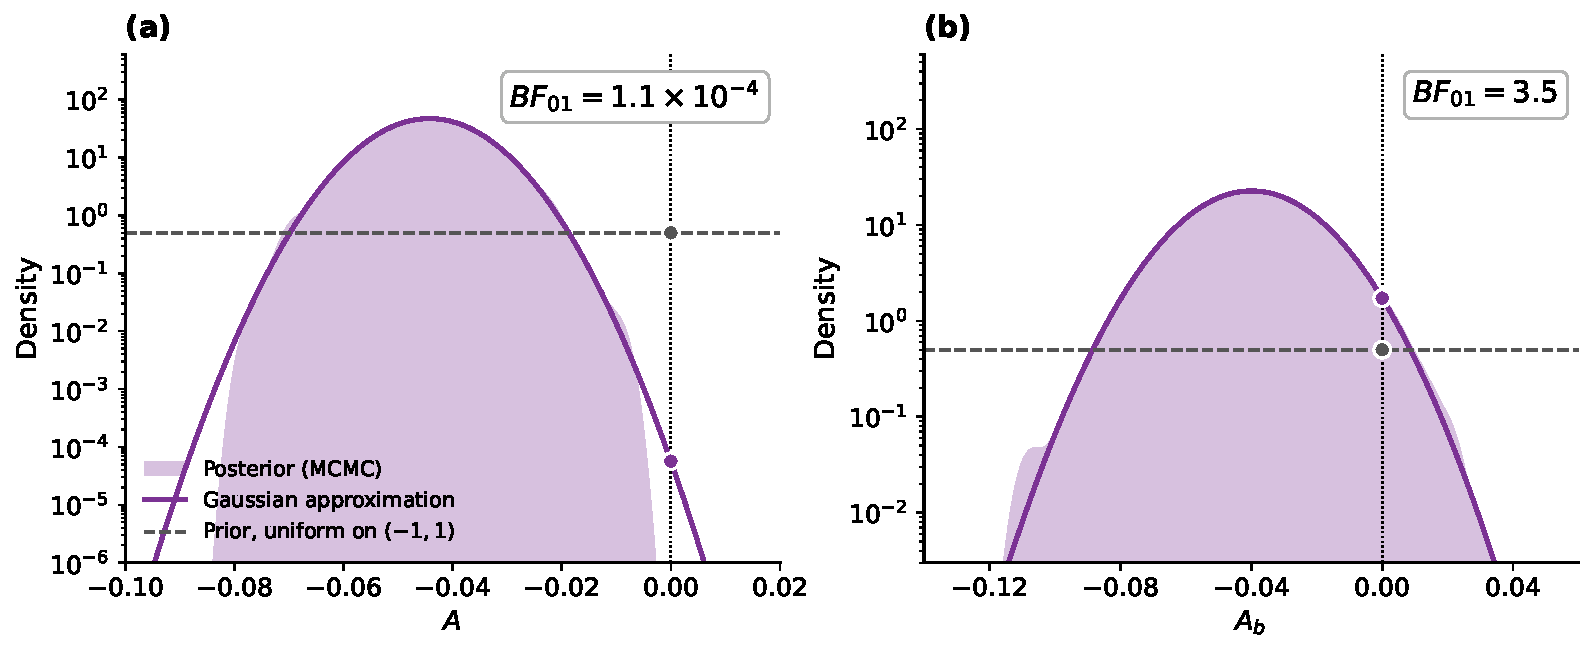
\includegraphics[width=0.95\textwidth]{figures/short_savage_dickey.pdf}
\caption{Savage-Dickey ratio for (a) $A$ and (b) $A_b$: marginal posterior (histogram of the chain and Gaussian approximation) and prior density, logarithmic scale. The Bayes factor $BF_{01}$ is the ratio of the two densities at zero (dots). For $A$ the posterior density at zero is $10^{-4}$ times the prior one; for $A_b$, $2.3$ standard deviations from zero, it is higher than the prior density, and the data favor $A_b=0$.}
\label{fig:bayes_sd}
\end{figure*}

\subsection{Priors and Bayes Factors}
\label{sec:checks_prior}
\emph{In short: no change of the prior on the nuisance parameters or of its parametrization moves $A$ by more than $0.0002$; the Bayes factor of $A=0$ scales with the prior width, and the evidence computed by direct integration agrees in order of magnitude with the Savage-Dickey ratio.}
The posterior was reweighted, without new sampling, to other priors: logarithmically uniform yields and slopes, a prior uniform in the lifetimes $1/\lambda$, and a prior flat in $(N_s^+,N_s^-)$ and $(N_b^+,N_b^-)$ instead of $(N_s,A)$ and $(N_b,A_b)$, which differ by the Jacobian $N_s/2$ (Table~\ref{tab:checks_prior}). The largest shift is $0.0002$, and the effective sample size of the reweighted chain is stated.

\begin{table}[h]
\centering
\resizebox{\ifdim\width>\linewidth\linewidth\else\width\fi}{!}{\begin{tabular}{lccc}
\toprule
Prior & $A$ (median) & $68\%$ interval & ESS \\
\midrule
Nominal (uniform) & $-0.0442$ & $[-0.0529,-0.0358]$ & $20000$ \\
Log-uniform $N_s$, $N_b$ & $-0.0442$ & $[-0.0529,-0.0358]$ & $19993$ \\
Log-uniform slopes & $-0.0440$ & $[-0.0528,-0.0356]$ & $12306$ \\
Uniform in $1/\lambda$ & $-0.0444$ & $[-0.0526,-0.0360]$ & $153$ \\
Flat in $(N_s^+,N_s^-)$ & $-0.0442$ & $[-0.0529,-0.0358]$ & $19999$ \\
Flat in $(N_s^\pm)$ and $(N_b^\pm)$ & $-0.0442$ & $[-0.0529,-0.0358]$ & $19993$ \\
\bottomrule
\end{tabular}}
\caption{Posterior of $A$ under alternative priors, by importance reweighting of the chain; ESS: effective sample size of the $20{,}000$ thinned samples.}
\label{tab:checks_prior}
\end{table}

The Bayes factor $BF_{01}=p(A=0\mid D)/\pi(0)$ is proportional to the density of the prior at zero, $\pi(0)=1/(2W)$ for a uniform prior on $(-W,W)$ (Fig.~\ref{fig:checks_bf}): for $A$ it stays below $10^{-2}$ for every width up to $W=1$ (decisive evidence for $A\neq0$ whatever the prior), while for $A_b$ it crosses $1$ at $W\simeq0.3$, which is the content of the Lindley paradox. The same evidence was computed by direct numerical integration over $A$ on a grid, $Z_1=\int L\,\pi\,dA$ with the nuisance parameters fixed at the maximum of the posterior, the method that is not feasible for twelve parameters: it gives $K_{01}=7.0e-05$, against $1.3e-04$ with the profile likelihood and $1.1e-04$ for the Savage-Dickey ratio, which marginalizes the nuisance parameters; the three values are of the same order and the conclusion is the same.


The Savage-Dickey ratio also tests the equality of the background shapes of the two charges, one parameter at a time, with the difference $\delta=\theta^+-\theta^-$: $BF_{01}=3.1$ for the steep slope $\lambda_1$ (difference at $0.8\sigma$), $2.2$ for $\lambda_2$ ($2.4\sigma$) and $1.1$ for the fraction $f$ ($2.0\sigma$). The data are not able to distinguish the shapes, with a weak preference for equal ones: this is why the variant with a shared shape moves $A$ by $-0.0037$ and is part of the systematic uncertainty, without being preferred.

\subsection{Model Adequacy: Goodness of Fit and Posterior Predictive Check}
\label{sec:bayes_gof}
\emph{In short: the model does not reach $\chi^2/\mathrm{ndof}\approx1$ ($164.1/88$), mainly because the signal tails are heavier than a Gaussian, but $\Araw$ changes by only $-0.0002$ with a Crystal Ball signal.}
\begin{table}[!t]
\centering
\begin{tabular}{lccc}
\toprule
Model & $\Araw$ & $\chi^2$/ndof & $p$ \\
\midrule
Nominal & $-0.0443$ & $164.1/88$ & $2\times10^{-6}$ \\
Crystal Ball signal & $-0.0445$ & $131.0/86$ & $1\times10^{-3}$ \\
$\mu$, $\sigma$ per charge & $-0.0443$ & $164.2/86$ & $8\times10^{-7}$ \\
Shared bkg.\ shape & $-0.0480$ & $174.1/91$ & $4\times10^{-7}$ \\
Symmetric bkg.\ ($A_b=0$) & $-0.0471$ & $169.8/89$ & $5\times10^{-7}$ \\
Single exponential & $-0.0480$ & $297.7/92$ & $2\times10^{-23}$ \\
\bottomrule
\end{tabular}
\caption{$\Araw$ (posterior median) and goodness of fit of the nominal model (Gaussian signal, double exponential per charge) and of the alternative signal and background models, same data and window.}
\label{tab:gof}
\end{table}


A binned comparison of data and posterior-median model ($\chi^2=\sum(\text{obs}-\text{exp})^2/\text{exp}$ over 50 bins of $10\,\MeV$ per charge, $100-12=88$ degrees of freedom) gives $\chi^2=164.1/88$ ($p=1.6\times10^{-6}$), with $95.4$ for $B^+$ and $68.7$ for $B^-$. The largest pulls, in the $B^+$ sample, sit on the two flanks of the peak, about $\pm3\sigma$ from $\mu$ (Fig.~\ref{fig:bayes_fit}): the observed signal shape has heavier tails than a Gaussian. Replacing the Gaussian by a Crystal Ball shape~\cite{skwarnicki}, a Gaussian core with a power-law low-mass tail,
\begin{equation}
S_{\mathrm{CB}}(x)\propto
\begin{cases}
e^{-x^2/2}, & x>-\beta,\\[2pt]
\left(\frac{\kappa}{\beta}\right)^{\kappa} e^{-\beta^2/2}\left(\frac{\kappa}{\beta}-\beta-x\right)^{-\kappa}, & x\leq-\beta,
\end{cases}
\label{eq:cb}
\end{equation}
with $x=(m-\mu)/\sigma$, $\beta$ the point where the tail starts (in units of $\sigma$) and $\kappa$ its power, both free, improves the fit to $\chi^2=131.0/86$ ($p=1.3\times10^{-3}$, $\beta=1.71$, $\kappa=35$) but moves $\Araw$ by only $-0.0002$ (Table~\ref{tab:gof}). The asymmetry does not depend on the signal shape even though none of the models reaches $\chi^2/\text{ndof}\approx1$. The Gaussian is nevertheless kept as the nominal signal model, common to the two analyses: the Crystal Ball adds two tail parameters that are poorly constrained (its power $\kappa$ runs to large values), and the effect of the signal shape on $\Araw$ is covered by the systematic study (Sec.~\ref{sec:syst}).

The background model is constrained by the data much more strongly. A single exponential per charge is rejected ($\chi^2=297.7/92$, $\Delta\chi^2=134$ for four fewer parameters), and so it is not used even as a systematic variant (Sec.~\ref{sec:syst}). A shape shared between the two charges ($\Delta\chi^2=10.0$ for three fewer parameters) and a charge-symmetric background ($\Delta\chi^2=5.7$ for one fewer) are acceptable descriptions and shift $\Araw$ by $-0.0037$ and $-0.0028$: the background treatment is the largest model dependence of the fit. The lower edge of the window is a compromise between two failures. Extending the window to $5050\,\MeV$ degrades the fit ($\chi^2=217.4/98$), because the double exponential no longer follows the background further below the peak; raising it to $5150\,\MeV$ removes most of the region that constrains the steep component, which becomes poorly identified -- the chain for its fraction $f_+$ mixes slowly ($N/\tau=10$) -- while $\Araw$ itself is unchanged ($-0.0444$).

\begin{figure*}[t]
\centering
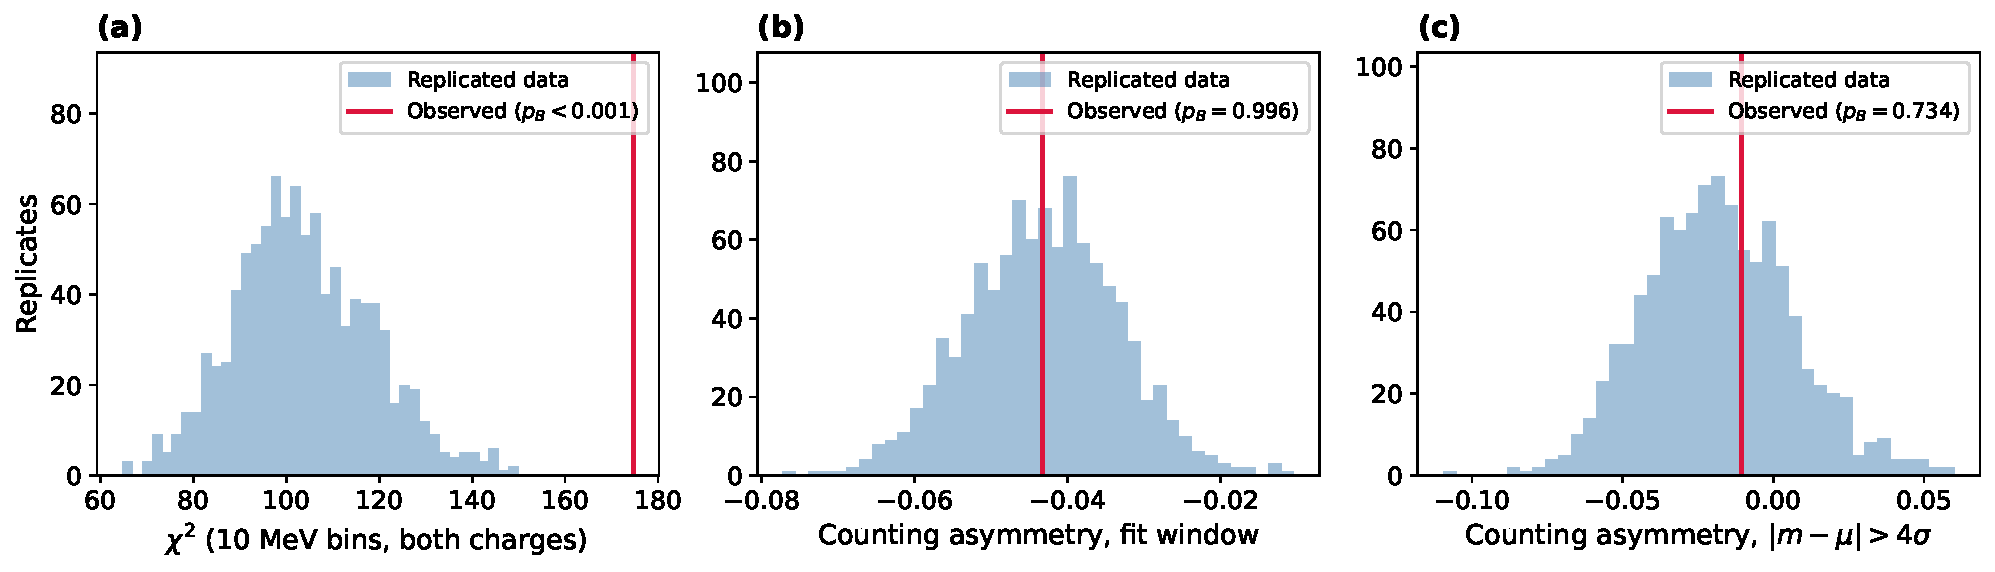
\includegraphics[width=0.95\textwidth]{figures/bayes_nominal_ppc.pdf}
\caption{Posterior predictive check: distributions of three discrepancies over $1000$ datasets replicated from posterior draws, compared with the observed values. (a) binned $\chi^2$; (b) and (c) counting asymmetry of the fit window and of the sidebands.}
\label{fig:bayes_ppc}
\end{figure*}

The binned $\chi^2$ uses the posterior medians only. A posterior predictive check~\cite{gelman_ppc} accounts for the posterior uncertainty and tests specific features of the data: for $1000$ parameter sets $\theta_j$ drawn from the posterior, a dataset $y^{\mathrm{rep}}_j$ is generated from the model, and a discrepancy $T(y,\theta_j)$ is computed both on the replica and on the data; the posterior predictive $p$-value is $p_B=P\big(T(y^{\mathrm{rep}},\theta)\geq T(y,\theta)\mid y\big)$. For the binned $\chi^2$ the replicas give $104\pm15$ and the data $175$ (median over $\theta_j$): none of the replicas reaches the observed value ($p_B<10^{-3}$), with the misfit concentrated in the $B^+$ sample ($p_B<10^{-3}$, against $0.03$ for $B^-$). The counting asymmetries of the whole window ($p_B=0.996$) and of the signal window ($0.99$) are reproduced, but this is expected and not informative: $A$ is a free parameter, so the replicas are centred on the observed value by construction. The asymmetry of the sidebands ($0.73$), which the fit constrains less directly, is also reproduced (Fig.~\ref{fig:bayes_ppc}). The check therefore shows that the model misdescribes the shape of the spectrum, mainly the signal tails, and does not reveal a charge-dependent distortion of the sidebands; that $\Araw$ does not depend on the signal shape is shown directly by its stability under the Crystal Ball model (Table~\ref{tab:gof}).

\subsection{Posterior Predictive Check with Statistics Not Fitted by the Model}
\label{sec:checks_ppc}
\emph{In short: the asymmetry in slices of the mass, which the model predicts, is reproduced ($p_B=0.67$), and the difference between the $\chi^2$ of the two charges is at the edge of the replicas ($p_B=0.08$).}
Section~\ref{sec:bayes_gof} noted that the counting asymmetries of the window are fitted by construction. Two statistics that are not adjusted directly were therefore used (Fig.~\ref{fig:checks_ppc}): the asymmetry in ten slices of $50\,\MeV$ of the mass against the one predicted by the model from the same posterior draw, which tests that the charge asymmetry follows the mixture of signal and background, $T=\sum_s(A_s-\bar A_s)^2/\sigma_s^2$, and the difference $\chi^2(B^+)-\chi^2(B^-)$ of the binned fit. The slice asymmetries are reproduced; the difference of the $\chi^2$ is $27$ in the data against $-0\pm15$ in the replicas, a $1.8\sigma$ excess that restates that the misfit is concentrated in the $B^+$ sample.

\begin{figure*}[t]
\centering
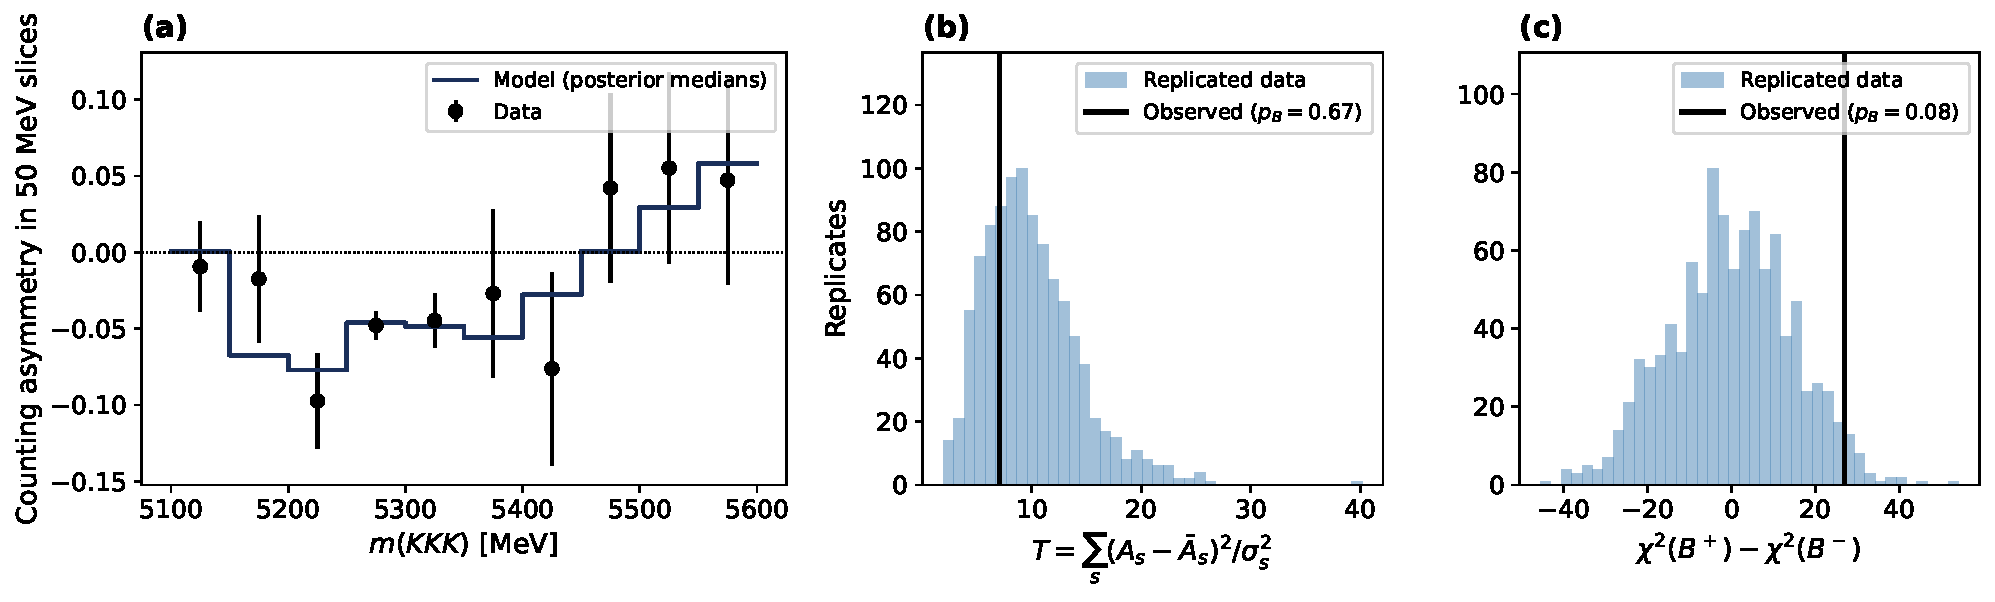
\includegraphics[width=0.95\textwidth]{figures/validation_ppc_unfitted.pdf}
\caption{(a) Counting asymmetry in slices of $50\,\MeV$ of the mass, data and model. (b) Distribution of $T=\sum_s(A_s-\bar A_s)^2/\sigma_s^2$ over $1000$ replicas and observed value. (c) The same for $\chi^2(B^+)-\chi^2(B^-)$.}
\label{fig:checks_ppc}
\end{figure*}

\subsection{Robustness Checks: Polarity, Prior and Charm Vetoes}
\label{sec:bayes_checks}
\emph{In short: $\Araw$ agrees between the two magnet polarities ($0.7\sigma$) and does not depend on the prior; the $D^0$ veto moves it by $2.3$ times the expected statistical spread.}
\begin{figure}[h]
\centering
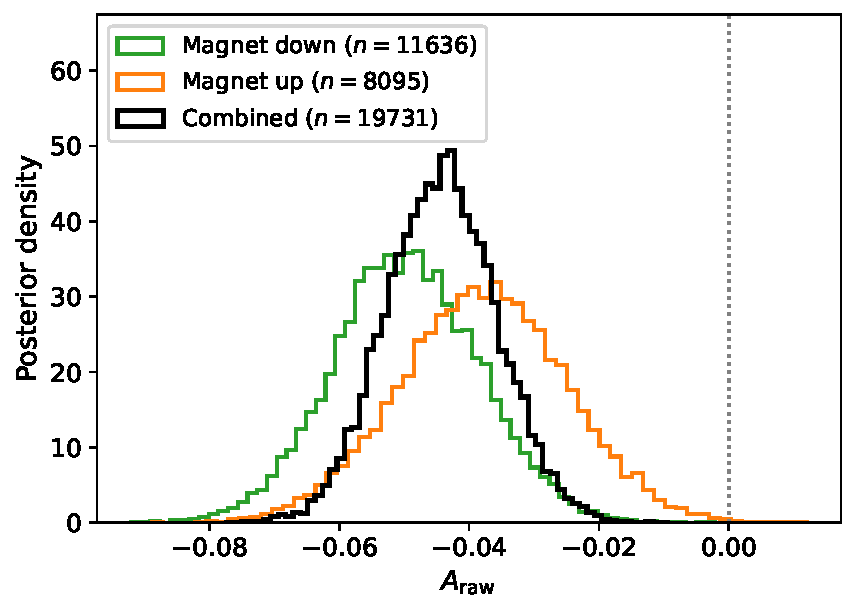
\includegraphics[width=\columnwidth]{figures/bayes_nominal_magnet.pdf}
\caption{Posterior of $\Araw$ for the magnet-down, magnet-up and combined samples.}
\label{fig:bayes_magnet}
\end{figure}

The fit was repeated separately on the two magnet polarities, whose left-right detection asymmetries are opposite and partially cancel in the combined sample: $\Araw(\text{down})=-0.0497\pm0.0112$ ($n=11{,}636$) and $\Araw(\text{up})=-0.0378\pm0.0129$ ($n=8095$); the Frequentist fits give $-0.0492\pm0.0111$ and $-0.0374\pm0.0131$, and the sum of their profile likelihoods $-0.0443\pm0.0084$ (Sec.~\ref{sec:checks_profile}). They differ by $0.7\sigma$, so there is no indication that the asymmetry is an artifact of one polarity (Fig.~\ref{fig:bayes_magnet}). A narrower prior, $A\in(-0.3,0.3)$, leaves the posterior unchanged ($\Araw=-0.0443$), as expected for a posterior far from the prior bounds; the prior width matters only for the Bayes factor (Sec.~\ref{sec:bayes_factor}).



The sample contains $B^\pm$ decays through intermediate charm states, $B^\pm\to D^0K^\pm$, $J/\psi K^\pm$ and $\chi_{c0}K^\pm$ with $D^0$, $J/\psi$, $\chi_{c0}\to K^+K^-$, which are visible as peaks in the opposite-sign $m(K^+K^-)$ spectra. They are part of the $B^\pm\to K^\pm K^+K^-$ final state and are kept in the nominal sample; removing them changes the observable, from the asymmetry of all $B^\pm\to K^\pm K^+K^-$ decays to that of the charmless ones, so the vetoes are reported as an informative check rather than as a systematic variation. A candidate is vetoed if either opposite-sign pair, $m(H1,H2)$ or $m(H1,H3)$, lies within $\pm30\,\MeV$ of the $D^0$ or $J/\psi$ mass or within $\pm60\,\MeV$ of the $\chi_{c0}$ mass (world-average masses; the wider window for the $\chi_{c0}$ reflects its natural width). The $D^0$ veto alone keeps $18{,}744$ candidates and gives $\Araw=-0.0496\pm0.0088$; the three vetoes together keep $16{,}367$ and give $-0.0423\pm0.0094$. The shifts with respect to the nominal fit, $-0.0053$ and $+0.0020$, compare with expected statistical fluctuations of $0.0023$ and $0.0040$ for a subsample of the nominal one (Sec.~\ref{sec:syst}); the $D^0$ veto moves $\Araw$ by $2.3$ times this amount, i.e.\ the vetoed $D^0K^\pm$ candidates have a less negative asymmetry than the rest of the sample. The analysis was also carried out with a minimal six-parameter model, with a narrower window and a single exponential background, before the nominal model was fixed; it gives a compatible result (Sec.~\ref{sec:bayes_minimal}).

\subsection{Toy-MC Coverage Validation}
\label{sec:bayes_toymc}
\emph{In short: $200$ toy-MC experiments give coverage $0.65\pm0.03$ ($68\%$) and $0.93\pm0.02$ ($95\%$), consistent with nominal, with unbiased estimates and pulls of width $1.04$.}
\begin{figure}[h]
\centering
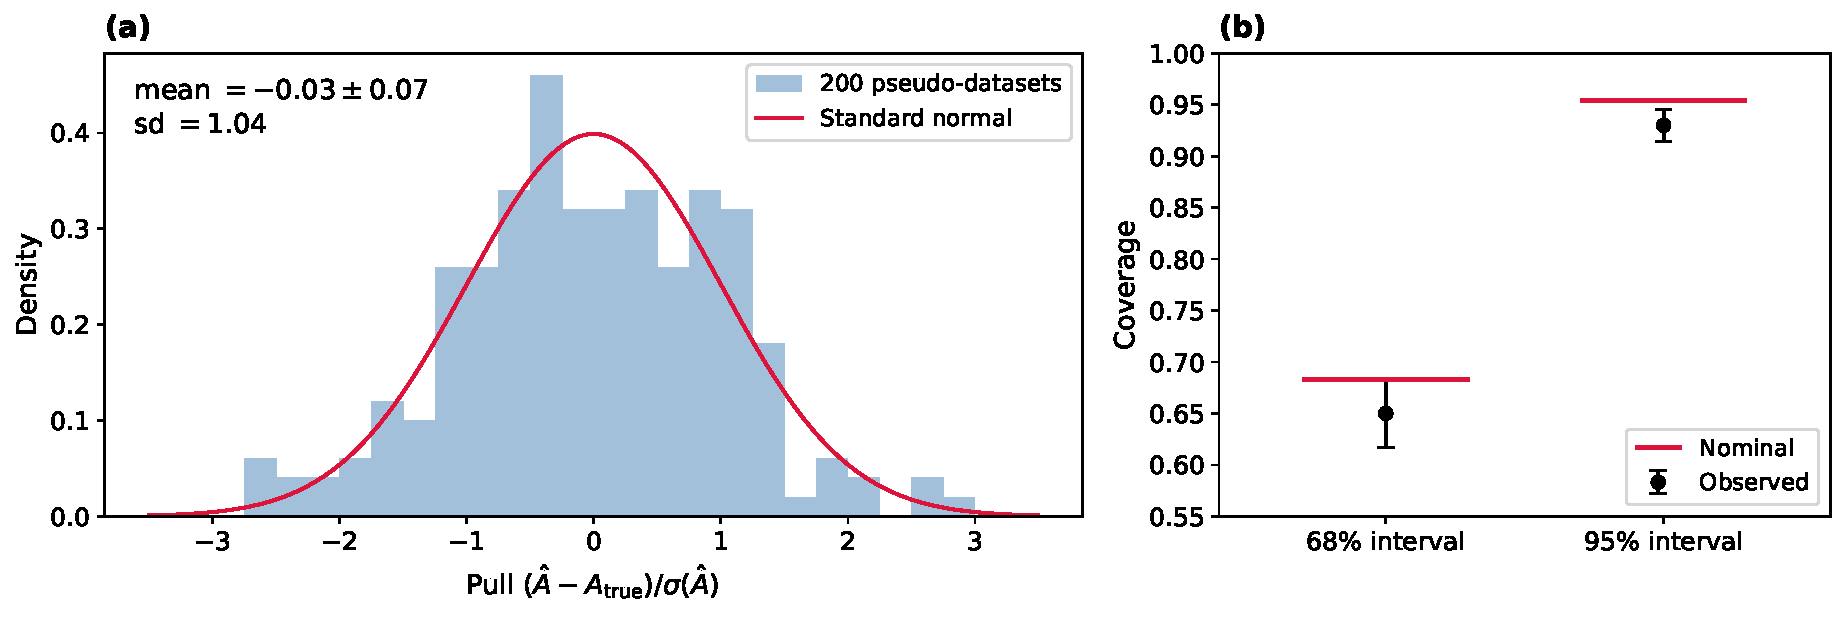
\includegraphics[width=\columnwidth]{figures/bayes_nominal_toys.pdf}
\caption{Toy-MC validation, 200 toy-MC datasets. (a) Pulls $(\hat A-A_{\mathrm{true}})/\sigma(\hat A)$, with $\hat A$ and $\sigma(\hat A)$ the posterior median and standard deviation of each replica, compared with a standard normal. (b) Fraction of replicas whose 68\% and 95\% credible intervals contain the injected value, with binomial uncertainties, and the nominal coverage.}
\label{fig:bayes_toys}
\end{figure}

A credible interval is a probability statement on $A$ given the data and the prior, whereas the nominal coverage of a confidence interval is a property of the procedure (Sec.~\ref{sec:frequentist}). With flat priors and $\sim2\times10^4$ events the two intervals coincide numerically (Sec.~\ref{sec:bayes_posterior}), but nothing guarantees the coverage of the credible interval, so it was checked: 200 toy-MC datasets were generated from the fitted model (parametric bootstrap, with the posterior medians as ground truth and Poisson-fluctuated yields for each charge and component; the truncated Gaussian and exponential masses are drawn with the transformation method, i.e.\ by inverting their cumulative distributions) and each was refit with the nominal procedure and a $12{,}000$-step chain. The fraction of replicas whose interval contains the injected $A$ is $0.650\pm0.033$ for the 68\% CI and $0.930\pm0.015$ for the 95\% CI (binomial uncertainties), $1.0\sigma$ and $1.3\sigma$ below nominal: the coverage is consistent with nominal. The estimates themselves are unbiased and their spread matches the reported uncertainty (Fig.~\ref{fig:bayes_toys}): their mean differs from the injected value by $-0.0002\pm0.0006$, their standard deviation, $0.0088$, agrees with the posterior standard deviation of the data fit, $0.0085$, and the pulls have mean $-0.03\pm0.07$ and standard deviation $1.04$.

The toy chains are shorter than the nominal one, and in 124 of the 200 replicas the slowest-mixing parameter, always a background-shape parameter, has $N/\tau<50$ (median $48$, minimum $22$). The criterion on the slowest parameter is conservative for the quantity tested here: for $A$ itself the median autocorrelation time is $156$ steps, so each chain is at least $45$ autocorrelation times long in $A$ and provides $\gtrsim1400$ effectively independent samples of it. The Monte Carlo error on the percentiles of $A$ is then a few per cent of $\sigma(A)$, negligible against the binomial uncertainty of the coverage, and the replicas with $N/\tau<50$ do not show a lower coverage than the others ($0.69$ for the $68\%$ interval, against $0.58\pm0.06$ for the $76$ replicas with $N/\tau\geq50$, whose coverage is $1.9$ standard deviations below nominal: the split was made after the fact and $200$ replicas cannot tell a trend from a fluctuation, and the check on the data of Sec.~\ref{sec:freq_coverage} gives the nominal coverage). This is a closure test of the inference procedure: since the toys are generated from the same model that is fitted, it does not probe the model mismatch of Sec.~\ref{sec:bayes_gof}, which is instead addressed by the systematic study.

\subsection{Metropolis-Hastings Sampler and Published Likelihood}
\label{sec:checks_mh}
\emph{In short: an own Metropolis-Hastings sampler reproduces the posterior of the ensemble sampler, and the profile likelihood is given in a table, so that the result can be combined with others.}
The algorithm of the ensemble sampler was replaced by the basic Metropolis-Hastings one: a Gaussian proposal with the covariance of the posterior scaled by $2.38^2/d$, $120{,}000$ steps with the first $1/6$ discarded. The acceptance is $0.24$, the integrated autocorrelation time of $A$ is $36$ steps ($2813$ effective samples), and $A=-0.0443$ with $68\%$ interval $[-0.0526,-0.0357]$, against $-0.0443$ and $[-0.0528,-0.0358]$ from the ensemble sampler: the two samplers give the same posterior.

The profile likelihood of $A$ is given in Table~\ref{tab:checks_qa}, together with the Minos intervals, so that other measurements of the same quantity can be combined with this one by adding $q(A)$.

\begin{table}[h]
\centering
\resizebox{\ifdim\width>\linewidth\linewidth\else\width\fi}{!}{\begin{tabular}{r|ccccccccc}
\toprule
$A$ & $-0.08$ & $-0.07$ & $-0.06$ & $-0.05$ & $-0.04$ & $-0.03$ & $-0.02$ & $-0.01$ & $+0.00$ \\
$q(A)$ & $17.9$ & $9.3$ & $3.5$ & $0.5$ & $0.2$ & $2.8$ & $8.1$ & $16.1$ & $27.0$ \\
\bottomrule
\end{tabular}}
\caption{Profile likelihood ratio $q(A)=-2\Delta\ln L$ of the nominal fit (other parameters profiled); minimum at $-0.0441$, Minos intervals $[-0.0526,-0.0356]$ ($68\%$) and $[-0.0607,-0.0275]$ ($95\%$).}
\label{tab:checks_qa}
\end{table}

\FloatBarrier
